\documentclass{beamer}
% September 2014
% Author: Dr Rachid Hourizi and Dr. Michael Wright 
% Department of Computer Science, University of Bath
\usepackage{listings}
\usetheme{Boadilla} 
\usepackage{fixltx2e}
\usepackage{hyperref}
\lstset{language=Java,,
	basicstyle=\ttfamily\small,
           keywordstyle=\color{blue}\ttfamily,
           stringstyle=\color{red}\ttfamily,
           commentstyle=\color{gray}\ttfamily,
          breaklines=true}

\begin{document}

\AtBeginSection[]{
  \begin{frame}
  \vfill
  \centering
  \begin{beamercolorbox}[sep=8pt,center,shadow=true,rounded=true]{title}
    \usebeamerfont{title}\insertsectionhead\par%
  \end{beamercolorbox}
  \vfill
  \end{frame}
}

\title{CM 10227: Lecture 7}
\author{Dr. Rachid Hourizi and Dr. Michael Wright}
\date{\today}
\frame{\titlepage}

\begin{frame}
\begin{center}
\textbf{Resources}
\end{center}
\begin{itemize}
\item More help with this course
\begin{itemize}
\item Moodle
\item E-mail - programming1@lists.bath.ac.uk
\end{itemize}
\item Online C \alert{and Java} IDE
\begin{itemize}
\item \url{https://www.codechef.com/ide}
\item Remember to select Java from the drop down menu.
\end{itemize}
\item Books
\begin{itemize}
\item Java by Dissection (Free pdf online)
\item The Java Tutorial (https://docs.oracle.com/javase/tutorial/)
\end{itemize}
\end{itemize}
\end{frame}

\begin{frame} 
\begin{itemize}
\item The places that you can get additional support if you are finding the pace of the course a little fast now include
\begin{itemize}
\item \text{The A labs}
\item \text{The B (catch up) lab}
\item \text{The Drop in Sessions}
\end{itemize}
\item please note that we have moved a couple of the labs
\item please check the details on Moodle and let us know if you now cannot get to a lab that you wold otherwise have attended.
\end{itemize}
\end{frame}

\begin{frame}
\begin{itemize}
\item If you struggling with the exercises, pace of the course and/or coding in general
\item Please come and see Rachid or Michael
\end{itemize}
\end{frame}
 
\begin{frame} 
\begin{itemize}
\item If, on the other hand, you are finding the pace a little slow  
\item You can still sign up for the Advanced Programming Labs
\end{itemize}
\end{frame}

\begin{frame}
\begin{center}
\textbf{Last time...}
\end{center} 
\begin{itemize}
\item First Classes and Objects
\end{itemize}
\end{frame}

\begin{frame}
\begin{center}
\textbf{This week}
\end{center} 
\begin{itemize}
\item (Almost) Reusing Code
\begin{itemize}
\item Inheritance
\item Polymorphism
\end{itemize}
\end{itemize}
\end{frame}

\begin{frame}
\begin{center}
\textbf{A Brief Recap}
\end{center}
\begin{itemize}
\item Java Classes (Templates)
\begin{itemize}
\item Fields
\item Constructors
\item Accessors and Mutators (Sometimes called Getters and Setters)

\end{itemize}
\end{itemize}
\end{frame}

\begin{frame}[fragile]
\small
\begin{block}{}
\begin{lstlisting}
public class Example{

}
\end{lstlisting}
\end{block}
\end{frame}

\begin{frame}[fragile]
\small
\begin{block}{}
\begin{lstlisting}
public class Example{
	private int exampleVariable;
}
\end{lstlisting}
\end{block}
\end{frame}

\begin{frame}[fragile]
\small
\begin{block}{}
\begin{lstlisting}
public class Example{
	private int exampleVariable;
	
	public Example(){
		exampleVariable = 1;
	}
}
\end{lstlisting}
\end{block}
\end{frame}

\begin{frame}[fragile]
\small
\begin{block}{}
\begin{lstlisting}
public class Example{
	private int exampleVariable;
	
	public Example(){
		exampleVariable = 1;
	}
	
	public Example(int value){
		exampleVariable = value;
	}
}
\end{lstlisting}
\end{block}
\end{frame}

\begin{frame}[fragile]
\small
\begin{block}{}
\begin{lstlisting}
public class Example{
	private int exampleVariable;
	
	public Example(){
		exampleVariable = 1;
	}
	
	public Example(int value){
		exampleVariable = value;
	}
	
	public void setExampleVariable(int value){
		exampleVariable = value;
	}
}
\end{lstlisting}
\end{block}
\end{frame}

\begin{frame}[fragile]
\small
\begin{block}{}
\begin{lstlisting}
public class Example{
	private int exampleVariable;
	
	public Example(){
		exampleVariable = 1;
	}
	
	public Example(int value){
		exampleVariable = value;
	}
	
	public void setExampleVariable(int value){
		exampleVariable = value;
	}
	
	public int getExampleVariable(){
		return exampleVariable;
	}
}
\end{lstlisting}
\end{block}
\end{frame}



\begin{frame}
\begin{center}
\textbf{Inheritance}
\end{center}
\end{frame}

\begin{frame}
\begin{itemize}
\item \textbf{Database of Multimedia Entertainment}
\item Stores details about Music Files and videos
\begin{itemize}
\item Music File: title, artist, \# tracks, playing time, got-it, comment
\item Video: title, director, playing time, got-it, comment
\end{itemize}
\item Allows (later) to search for information or print lists
\end{itemize}
\end{frame}

\begin{frame}
\frametitle{DOME Object Diagram}
\begin{center}
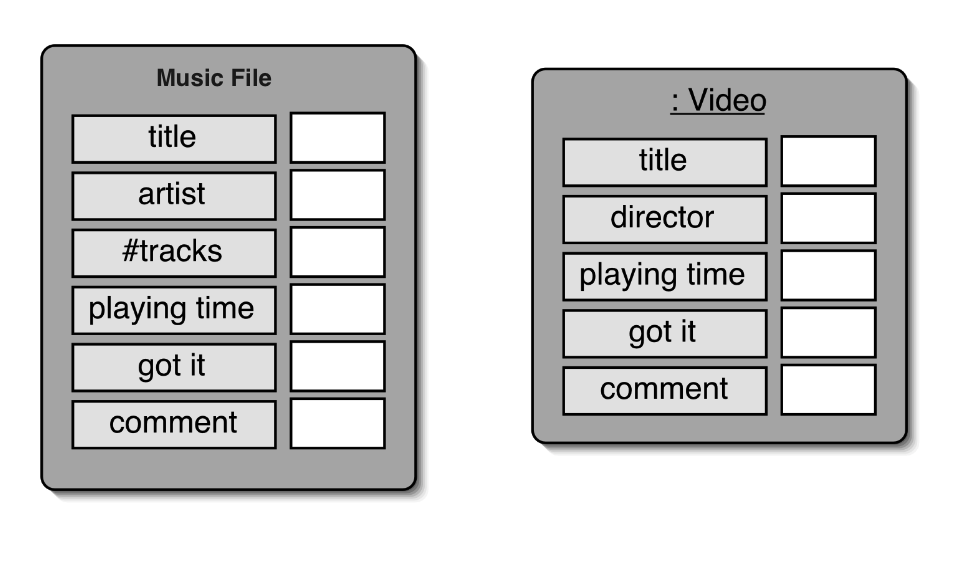
\includegraphics[height=5cm, keepaspectratio]{images/domeobjectdiagram}
\end{center}
\end{frame}

\begin{frame}
\frametitle{DOME Class Diagram}
\begin{center}
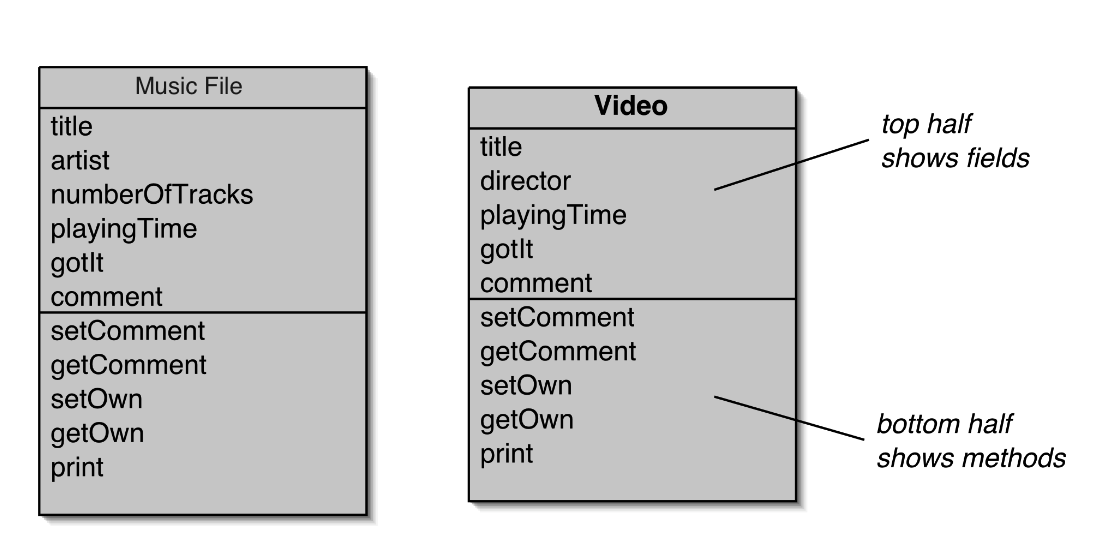
\includegraphics[height=5cm, keepaspectratio]{images/domeclassdiagram}
\end{center}
\end{frame}

\begin{frame}
\frametitle{DOME Object Diagram continued...}
\begin{center}
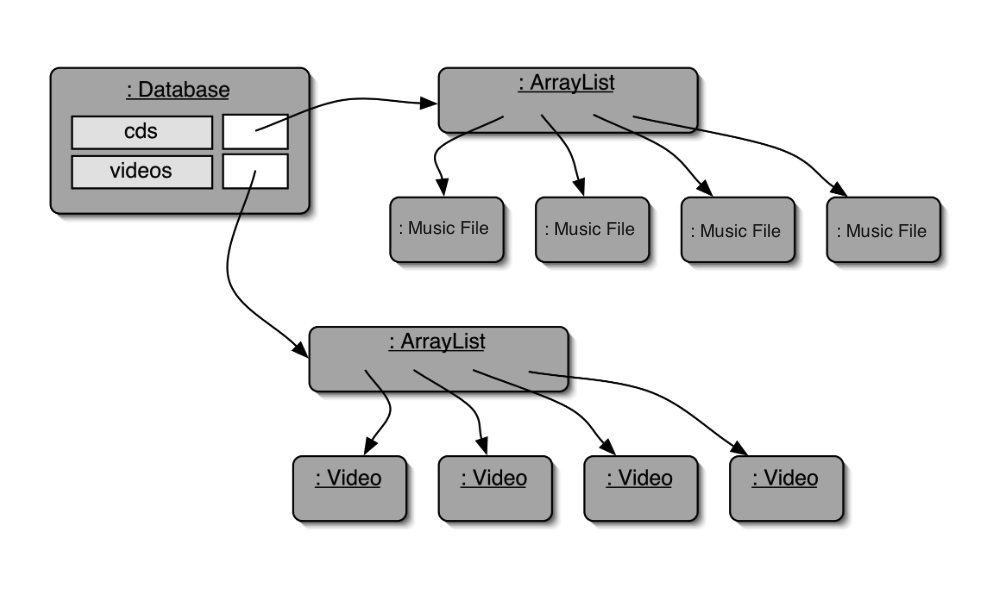
\includegraphics[height=5cm, keepaspectratio]{images/domeobjectdiagram2}
\end{center}
\end{frame}

\begin{frame}
\frametitle{DOME Class Diagram continued...}
\begin{center}
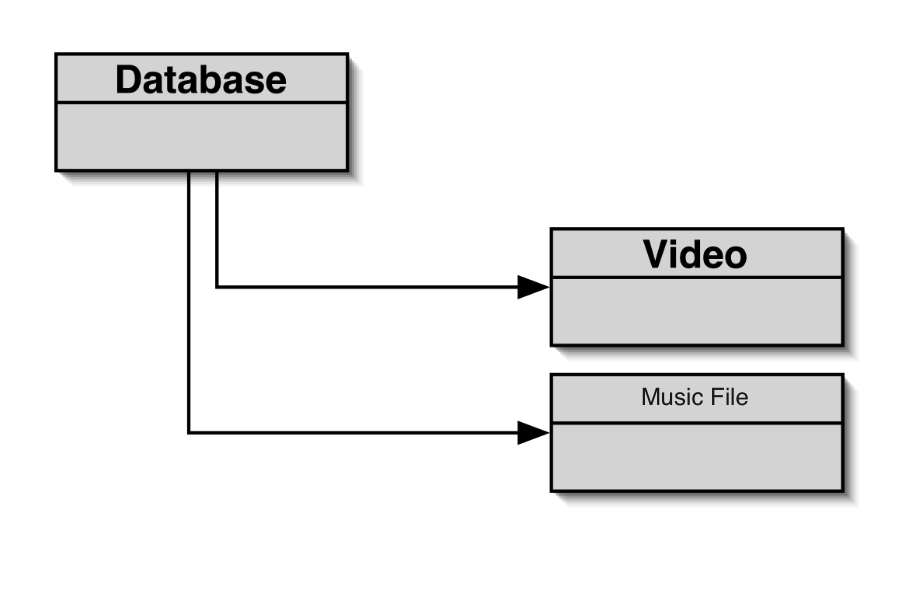
\includegraphics[height=5cm, keepaspectratio]{images/domeclassdiagram2}
\end{center}
\end{frame}

\begin{frame}[fragile]
\begin{block}{}
\begin{lstlisting}
public class MusicFile {
  private String title ; 
  private String artist ; 
  private String comment;

  public MusicFile( String theTitle , String theArtist ) {
  title = theTitle; 
  artist = theArtist; 
  comment = "";
  }

  public void setComment (String newComment)  {...}

  public String getComment()  {...}

  public void print ()  {...}
  
}
\end{lstlisting}
\end{block}
\end{frame}

\begin{frame}[fragile]
\begin{block}{}
\begin{lstlisting}
public class Video{
  private String title ; 
  private String director ; 
  private String comment;	

  public Video( String theTitle, String theDirect ){
    title = theTitle;
    director=theDirect;
    comment="";
  }	

  public void setComment(String newComment) { ... }

  public String getComment() { ... }

  public void print()  { ... }	

}
\end{lstlisting}
\end{block}
\end{frame}

\begin{frame}[fragile]
\begin{block}{}
\begin{lstlisting}
public class Database{
  private ArrayList MusicFiles;
  private ArrayList videos;

  public void list(){
	
    for(i=0, i<MusicFiles.size(); i++){
      MusicFile.get(i).print();
      System.out.println();
    }
    	
    for(i=0, i<videos.size(); i++){
      videos.get(i).print();
      System.out.println();	
    } 
  }	
}	
\end{lstlisting}
\end{block}
\end{frame}

\begin{frame}
\begin{itemize}
\item Critique of DOME
\end{itemize}
\begin{itemize}
\item Code duplication
\begin{itemize}
\item MusicFile and Video classes very similar (large part are identical)
\item makes maintenance difficult/more work
\item introduces danger of bugs through incorrect maintenance
\end{itemize}
\item Code duplication also in Database class 
\end{itemize}
\end{frame}

\begin{frame}
\frametitle{DOME Object Diagram Using Inheritance}
\begin{center}
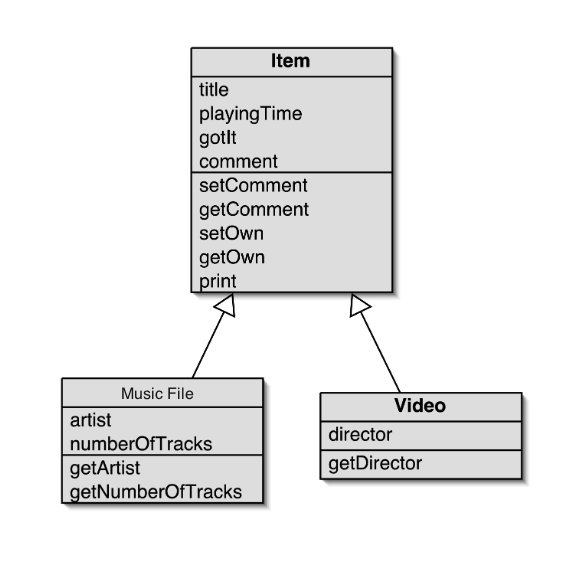
\includegraphics[height=8cm, keepaspectratio]{images/inheritance}
\end{center}
\end{frame}

\begin{frame}
\begin{itemize}
\item Using Inheritance
\begin{itemize}
\item define one superclass : Item
\item define subclasses for Video and MusicFile
\item the superclass defines common attributes
\item the subclasses inherit the superclass attributes
\item the subclasses add own attributes
\end{itemize}
\end{itemize}
\end{frame}

\begin{frame}
\frametitle {Object Diagram Using Inheritance}
\begin{center}
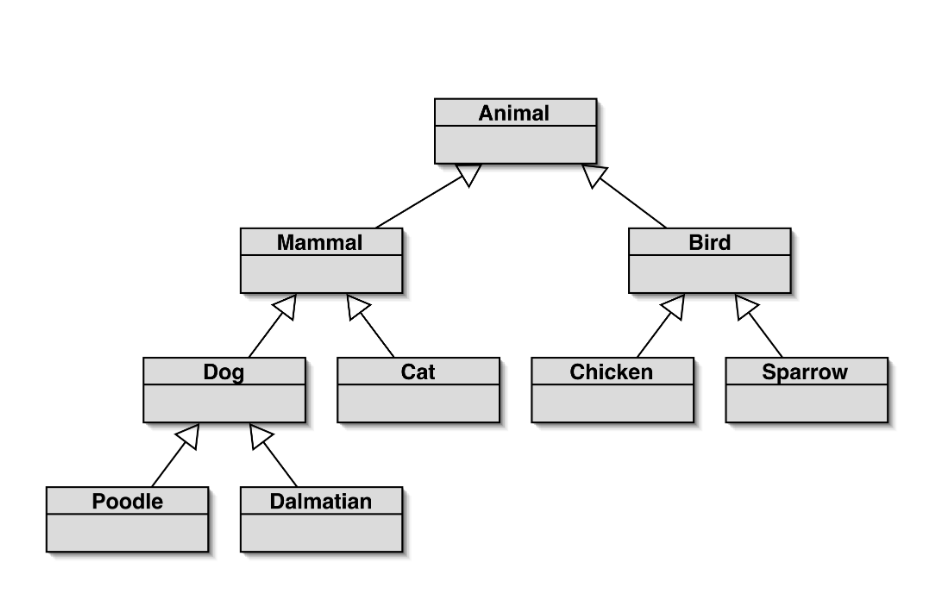
\includegraphics[height=7cm, keepaspectratio]{images/inheritance2}
\end{center}
\end{frame}

\begin{frame}[fragile]
\begin{block}{}
\begin{lstlisting}

public class Item{
  private String title ; 
  private int playingTime ; 
  private boolean gotIt ; 
  private String comment;

  //constructors and methods omitted...
}
\end{lstlisting}
\end{block}
\end{frame}

\begin{frame}[fragile]
\begin{block}{}
\begin{lstlisting}
public class MusicFile extends Item{
	
  private String artist;
  private int numberOfTracks;
	
  //constructors and methods omitted	
	
}
\end{lstlisting}
\end{block}

\begin{block}{}
\begin{lstlisting}
public class Video extends Item{
	
  private String director;
	
  //constructors and methods omitted	
	
}
\end{lstlisting}
\end{block}
\end{frame}

\begin{frame}[fragile]
\small
\begin{block}{}
\begin{lstlisting}
public class Item{
	
  private String Title;
  private int playingTime;
  private boolean gotIt;
  private String comment;

  public Item(Sring theTitle, int time){
    title = theTitle;
    playingTime = time;
    gotIt = false;
    comment = "";	
  }	

  //methods omitted
 
}
\end{lstlisting}
\end{block}
\end{frame}

\begin{frame}[fragile]
\begin{block}{}
\begin{lstlisting}
public class MusicFile extends Item{
  private String artist;
  private int numberOfTracks;

  public MusicFile(String theTitle, String theArtist,
  		 int tracks, int time){
    super(theTitle, time);
    artitst = theArtist;
    numberOfTracks = tracks;
  } 
 
  //methods omitted
 
}
\end{lstlisting}
\end{block}
\end{frame}

\begin{frame}
\begin{itemize}
\item Subclass constructors must always contain a 'super' call.
\begin{itemize}
\item If none is written, the compiler inserts one (without parameters)
\item Works only, if the superclass has a constructor without parameters
\item Must be the first statement in the subclass constructor.
\end{itemize}
\end{itemize}
\end{frame}

\begin{frame}[fragile]
\begin{block}{}
\begin{lstlisting}
public class Database {
  private ArrayList<Item> items ;
  ��
  // Construct an empty Database
  public Database( ) {
    items = new ArrayList<Item>() ; 
  }

  // Add an item to the database
  public void addItem ( Item theItem ) {
    items.add(theItem);
  }
  ...
}
\end{lstlisting}
\end{block}
\url{http://docs.oracle.com/javase/7/docs/api/java/util/ArrayList.html}
\end{frame}

\begin{frame}[fragile]
\begin{block}{}
\begin{lstlisting}
/**
* Print a list of all currently stored MusicFiles and 
* videos to the text terminal .
**/

public void list () {
  for(i=0; i<items.size; i++){ 
    Item item = items.get(i);
    item.print();
    System.out.println() ;   
  } 
}
\end{lstlisting}
\end{block}
\end{frame}

\begin{frame}[fragile]
\begin{itemize}
\item Subtyping
\bigskip
\item First, we had:
\begin{itemize}
\item public void addMusicFile(MusicFile theMusicFile)
\item public void addVideo(Video theVideo)
\end{itemize}
\item Now, we have:
\begin{itemize}
\item public void addItem(Item theItem)
\item We call this method with:
\end{itemize}
\end{itemize} 

\begin{block}{}
\begin{lstlisting}
Video myVideo = new Video(...);
database.addItem(myVideo);
\end{lstlisting}
\end{block}
\end{frame}

\begin{frame}
Subclasses and subtyping
\begin{itemize}
\item Classes define types.
\item Subclasses define subtypes.
\item Objects of subclasses can be used where objects of supertypes are required.
\item This is called substitution.
\end{itemize}
\end{frame}

\begin{frame}[fragile]
\begin{itemize}
\item Subclass objects may be assigned to superclass variables
\item e.g. Car extends Vehicle and Bicycle extends Vehicle
\end{itemize}
\begin{block}{}
\begin{lstlisting}
Vehicle v1 = new Vehicle();
Vehicle v2 = new Car();
Vehicle v3 = new Bicycle();
\end{lstlisting}
\end{block}
\end{frame}

\begin{frame}[fragile]
\begin{itemize}
\item Subclass objects may be passed to superclass parameters
\end{itemize}
\begin{block}{}
\begin{lstlisting} 

public class Database{
  public void addItem (Item theItem){
    ....
  }
}

//code in another method
Video video = new Video(...); 
MusicFile MusicFile = new MusicFile(...);

database.addItem (video); 
database.addItem (MusicFile);
\end{lstlisting}
\end{block}
\end{frame}

\begin{frame}
\frametitle{Object Diagram Illustrating Inheritance}
\begin{center}
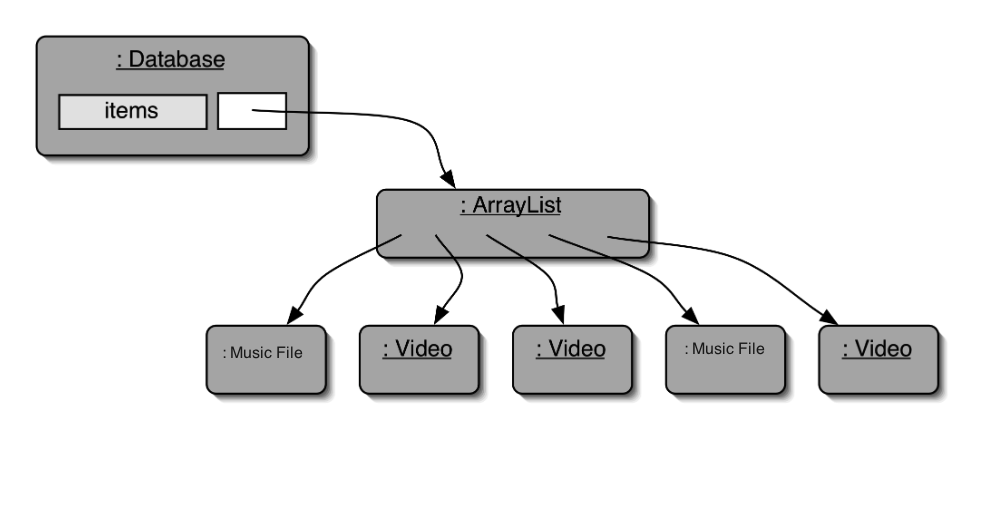
\includegraphics[height=6cm, keepaspectratio]{images/inheritance3}
\end{center}
\end{frame}

\begin{frame}
\frametitle{Class Diagram Illustrating Inheritance}
\begin{center}
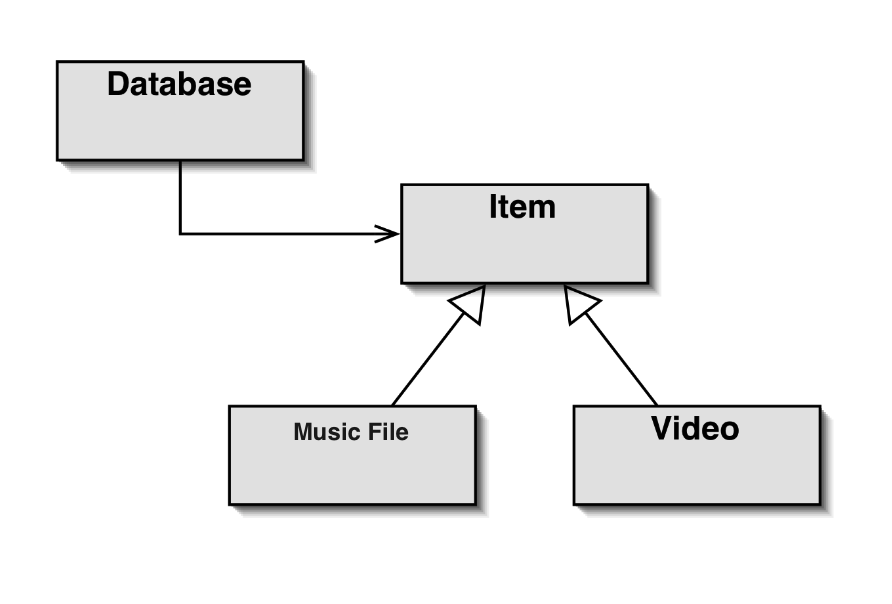
\includegraphics[height=7cm, keepaspectratio]{images/inheritance4}
\end{center}
\end{frame}

\begin{frame}
Review
\begin{itemize}
\item Inheritance allows the definition of classes as extensions of other classes.
\item Inheritance
\begin{itemize}
\item avoids code duplication
\item allows code reuse
\item simplifies the code
\item simplifies maintenance and extending
\end{itemize}
\item Variables can hold subtype objects.
\item Subtypes can be used wherever supertype objects are expected (substitution).
\end{itemize}
\end{frame}

\begin{frame}
\begin{itemize}
\item Polymorphic variables
\item Object variables in Java are polymorphic.
\begin{itemize}
\item They can hold objects of more than one type.
\end{itemize}
\item They can hold objects of the declared type, or of subtypes of the declared type.
\end{itemize}
\end{frame}

\begin{frame}
\begin{center}
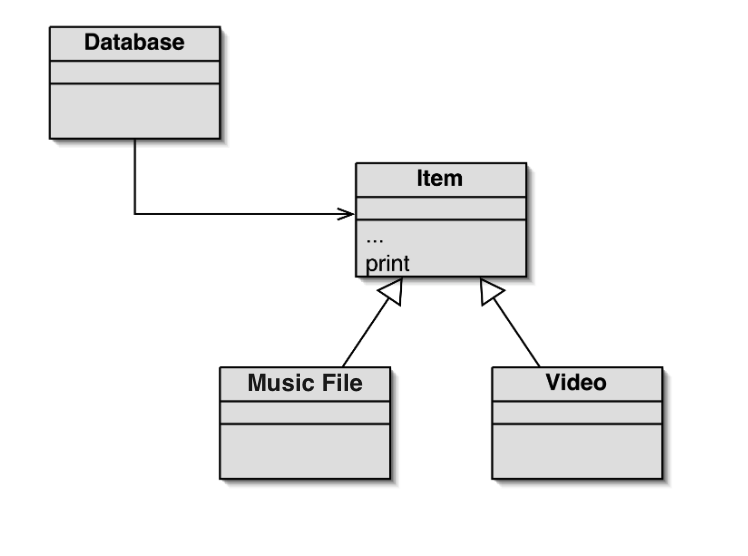
\includegraphics[height=6cm, keepaspectratio]{images/poly}
\end{center}
\end{frame}

\begin{frame}
\begin{itemize}
\item The print method in Item only prints the common fields.
\item Inheritance is a one-way street:
\bigskip
\item A subclass inherits the superclass fields.
\item The superclass knows nothing about its subclasss fields.
\end{itemize}
\end{frame}

\begin{frame}
\begin{itemize}
\item Attempting to Solve the Problem.
\bigskip
\item Place print where it has access to the information it needs.
\begin{center}
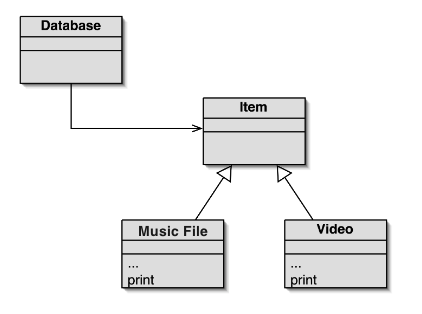
\includegraphics[height=6cm, keepaspectratio]{images/poly2}
\end{center}
\end{itemize}
\end{frame}

\begin{frame}
\begin{itemize}
\item Each subclass has its own version.
\item But Items fields are private.
\item Database cannot find a print method in Item.
\end{itemize}
\end{frame}

\begin{frame}
\begin{itemize}
\item To solve our problem we need to introduce...
\item some new terminology:
\begin{itemize}
\item static type
\item dynamic type
\item method dispatch/lookup
\end{itemize}
\end{itemize}
\end{frame}

\begin{frame}[fragile]
\begin{itemize}
\item Static Type and Dynamic Type
\item The declared type of a variable is its static type.
\item The type of the object a variable refers to is its dynamic type.
\item The compilers job is to check for static-type violations.
\end{itemize} 
\end{frame}

\begin{frame}[fragile]
\begin{block}{}
\begin{lstlisting}
class Alpha{}
class Beta extends Alpha{}
class Fruit extends Beta{}

Fruit f = new Fruit(); //static=Fruit, dynamic=Fruit
Alpha a = f; //static=Alpha, dynamic=Fruit

Fruit f = a //static type violation

\end{lstlisting}
\end{block}
\end{frame}

\begin{frame}
\begin{itemize}
\item Returning to our problem...
\item The Solution: Overriding
\begin{itemize}
\item print method in both super- and subclasses
\item Satisfies both static and dynamic type checking
\end{itemize}
\end{itemize}
\end{frame}

\begin{frame}
\begin{center}
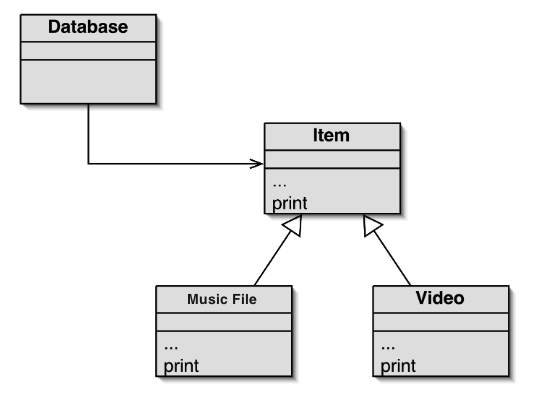
\includegraphics[height=6cm, keepaspectratio]{images/poly3}
\end{center}
\end{frame}

\begin{frame}
\begin{itemize}
\item Superclass and subclass define methods with the same signature.
\item Each has access to the fields of its class.
\item Superclass satisfies static type check.
\item Subclass method is called at runtime it overrides the superclass version.
\item What becomes of the superclass version?
\end{itemize}
\end{frame}

\begin{frame}
\begin{itemize}
\item Method Lookup 1
\begin{itemize}
\item No inheritance or polymorphism.
\item The obvious method is selected.
\end{itemize}
\end{itemize}
\begin{center}
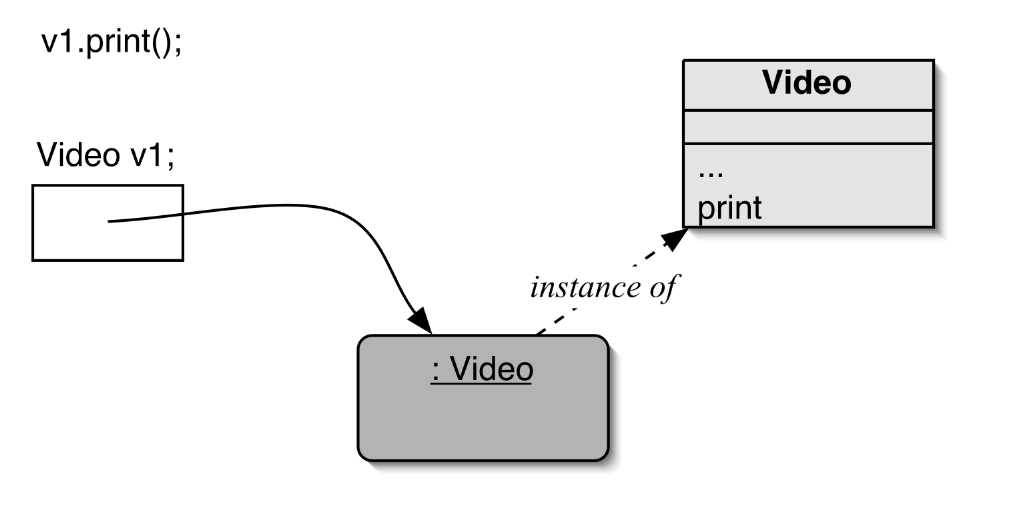
\includegraphics[height=5cm, keepaspectratio]{images/poly4}
\end{center}
\end{frame}

\begin{frame}
\begin{itemize}
\item Method Lookup 2
\begin{itemize}
\item Inheritance but no overriding
\item The inheritance hierarchy is ascended, searching for a match.
\end{itemize}
\end{itemize}
\begin{center}
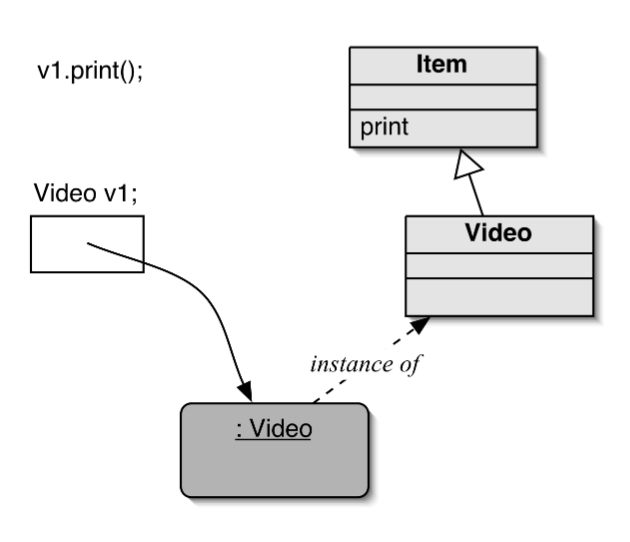
\includegraphics[height=5cm, keepaspectratio]{images/poly6}
\end{center}
\end{frame}

\begin{frame}
\begin{itemize}
\item Method Lookup 3
\begin{itemize}
\item Polymorphism and overriding.
\item The first version found is used.
\end{itemize}
\end{itemize}
\begin{center}
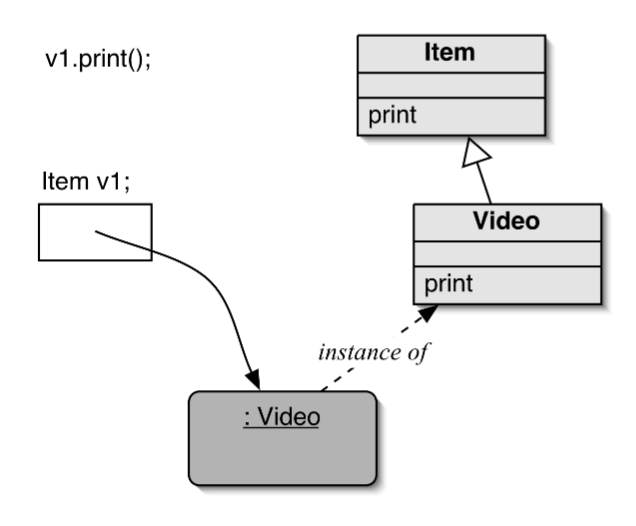
\includegraphics[height=5cm, keepaspectratio]{images/poly5}
\end{center}
\end{frame}\begin{frame}


Method Lookup Summary
\begin{itemize}
\item The variable is accessed.
\item The object stored in the variable is found.
\item The class of the object is found.
\item The class is searched for a method match.
\item If no match is found, the superclass is searched.
\item This is repeated until a match is found, or the class hierarchy is exhausted.
\item Overriding methods take precedence.
\end{itemize}
\end{frame}

\begin{frame}
\begin{itemize}
\item Super call in methods
\item Overridden methods are hidden ...
\item ... but we often still want to be able to call them.
\item An overridden method can be called from the method that overrides it
\begin{itemize}
\item super.method(...)
\item Compare with the use of super in constructors.
\end{itemize}
\end{itemize}
\end{frame}

\begin{frame}[fragile]
\begin{block}{}
\begin{lstlisting}
public class MusicFile{

  ...

  public void print (){
    super.print();
    System.out.println (""+artist);
    System.out.println("tracks:" + numberofTracks);
  }
}
\end{lstlisting}
\end{block}
\end{frame}

\begin{frame}
\begin{itemize}
\item We have been discussing polymorphic method dispatch.
\item A polymorphic variable can store objects of varying types.
\item Method calls are polymorphic.
\begin{itemize}
\item The actual method called depends on the dynamic object type.
\end{itemize}
\end{itemize}
\end{frame}

\begin{frame}
\begin{itemize}
\item Methods in Object are inherited by all classes.
\item Any of these may be overridden.
\item The toString method is commonly overridden:
\item public String toString()
\begin{itemize}
\item Returns a string representation of the object.
\end{itemize}
\end{itemize}
\end{frame}

\begin{frame}[fragile]
\begin{block}{}
\begin{lstlisting}
public class Item{
	
 ...
 
  public String toString (){
    String line1=title + " : " + playingTime + " mins");
    if(gotIt) {
      return line1 + "\n" + comment + "\n"); 
    } 
    else {
      return line1 + "\n" + comment + " need to buy" + "\n");
    }
  }
}
\end{lstlisting}
\end{block}
\end{frame}

\begin{frame}[fragile]
\begin{itemize}
\item Explicit print methods can often be omitted from a class:
\end{itemize}
\begin{block}{}
\begin{lstlisting}
System.out.println(item.toString()) ;
\end{lstlisting}
\end{block}
\begin{itemize}
\item Calls to println with just an object automatically result in
\item toString being called:
\end{itemize}
\begin{block}{}
\begin{lstlisting}
System.out.println(item);
\end{lstlisting}
\end{block}
\end{frame}

\begin{frame}
\begin{itemize}
\item Private access in the superclass may be too restrictive for a subclass.
\item The closer inheritance relationship is supported by protected access.
\item Protected access is more restricted than public access.
\item We still recommend keeping fields private.
\item Define protected accessors and mutators.
\end{itemize}
\end{frame}

\begin{frame}
\begin{center}
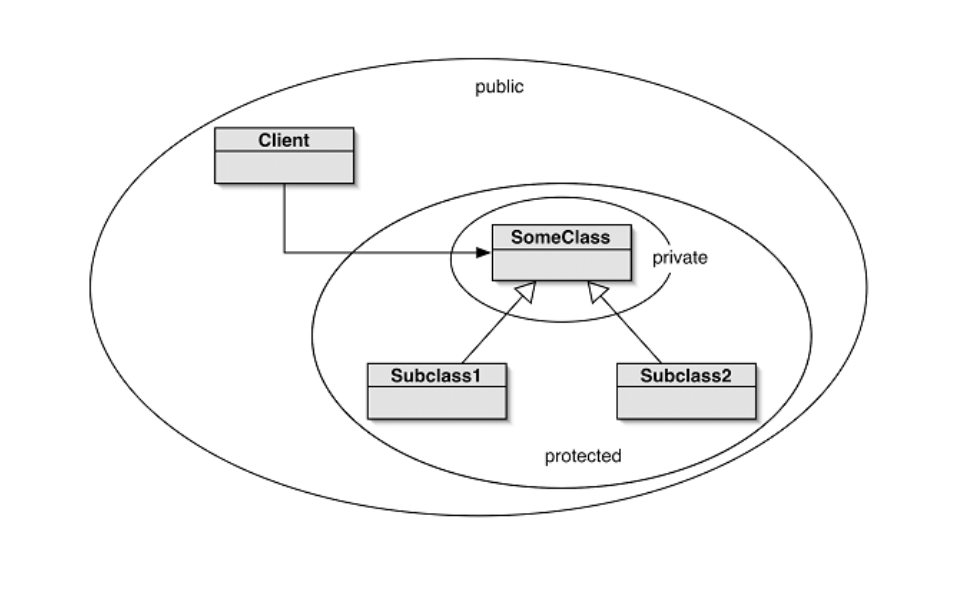
\includegraphics[height=8cm, keepaspectratio]{images/access}
\end{center}
\end{frame}

\begin{frame}
\begin{itemize}
\item Review
\bigskip
\item The declared type of a variable is its static type.
\item Compilers check static types.
\item The type of an object is its dynamic type.
\item Dynamic types are used at runtime.
\item Methods may be overridden in a subclass.
\item Method lookup starts with the dynamic type.
\item Protected access supports inheritance.
\end{itemize}
\end{frame}




\end{document}